\documentclass[12pt]{article}
\usepackage[utf8]{inputenc}
%\usepackage[T1,T2A]{fontenc}
\usepackage[T2A]{fontenc}
\usepackage[serbian]{babel}
\usepackage{geometry}
\geometry{margin=1in}
%\usepackage{helvet}
%\usepackage{avant}
%\renewcommand{\familydefault}{\sfdefault}
\usepackage{graphicx}
\usepackage{multicol}
\usepackage[document]{ragged2e}
\usepackage{fancyhdr}
\usepackage{hyperref}
\usepackage[svgnames]{xcolor}
\usepackage{caption}

%\newcommand{\mycode}[1]{\texttt{\colorbox{LightGrey}{#1}}}
\newcommand{\mycode}[1]{\texttt{\colorbox{Lavender}{#1}}}

\hypersetup{
    colorlinks=true,
    linkcolor=black,
    filecolor=black,      
    urlcolor=blue,
    }

\pagestyle{fancy}
\fancyhf{}
\fancyhead[L]{Основи машинског и дубоког учења}
%\fancyhead[C]{Top Center}
\fancyhead[R]{документација}
\renewcommand{\headrulewidth}{0.4pt}
%\fancyfoot[L]{Bottom Left}
\fancyfoot[C]{\thepage}
%\fancyfoot[R]{Bottom Right}
\renewcommand{\footrulewidth}{0.4pt}

\addto\captionsserbian{\renewcommand*\contentsname{Садржај:}}
%\setcounter{tocdepth}{2}

%\setlength\parindent{24pt}

\begin{document}
\thispagestyle{empty}
\begin{center}
\Large{
Универзитет у Крагујевцу
\vspace{0.3cm}\\
Факултет инжењерских наука
}
\vspace{0.7cm}\\

\includegraphics{images/fin_image}
\vspace{0.7cm}\\
\LARGE{
Документација за пројекат из предмета:
\vspace{0.1cm}\\
Основи машинског и дубоког учења
}
\vspace{1cm}\\
\LARGE{
\textbf{Тема:}
\vspace{0.3cm}\\
Аутономна вожња формула имплементирана као видео игра коришћењем учења подстицајем
}
\vspace{2.5cm}
\end{center}

\begin{tabular}{cc}
Студенти:\\
Михаило Максимовић 602/2018\\
Ђорђе Гачић 626/2018\\
\end{tabular}
\setlength{\tabcolsep}{12em}
\begin{tabular}{cc}
Професор:\\
Др Владимир Миловановић\\
Асистент:\\
Никола Радовановић\\
\end{tabular}
\begin{center}
\vspace{1cm}
Крагујевац, фебруар 2022.
\end{center}
\newpage

\tableofcontents
\newpage

\section{Увод}
\justifying
Машинско учење је подобласт вештачке интелигенције чији је циљ конструисање алгоритама и рачунарских система који су способни да  се адаптирају на нове ситуације и уче на бази искуства. Развијене су различите технике учења за извршавање различитих задатака. У овоме пројекту биће разматрана техника учења подстицајем (енг. Reinforcement Learning) кроз имплементацију у видео игри трке формула. Учење подстицајем је област машинског учења која се бави изучавањем начина на који интелигентни агенти треба да предузму акције у окружењу како би максимизирали појам кумулативне награде. \\
\indentУчење подстицајем је једна од три основне парадигме машинског учења, поред надгледаног и ненадгледаног учења. Изучавањем технике учења подстицајем развили су се многи занимљиви и корисни пројекти тако да је ова техника постала веома популарна и ушла у широку употребу.\\ 
\indentМотивација за израду овог пројекта била је идеја аутономне вожње. Кроз трку болида који самостално возе, на неком вишем нивоу од овог пројекта, могу се организовати такмичења научених модела што може бити веома занимљиво ако би се спровело у пракси. У наставку ће бити објашњене тахнологије коришћене при изради пројекта као и начин на који је пројекат имплементиран.\\
\indentИдеја пројекта је да се особа која игра игру и управља једном формулом утркује са осталим формулама које представљају утрениране моделе. 

\newpage
\section{Опис коришћене технологије}
\subsection{Списак коришћене технологије}
\indentЗа израду пројекта коришћене су следеће технологије:
\begin{itemize}
  \item Оперативни систем: Windows 10.
  \item Unity - мулти-платформски софтвер за израду игара који данас подржава развој на десктоп, мобилним и конзолним платформама, као и на платформама за виртуелну реалност.
  \item ML-Agents - пројекат отвореног кода који омогућава играма и симулацијама да служе као окружења за обуку интелигентних агената. Пружа имплементације најсавременијих алгоритама (засновани на PyTorch-у) како би се омогућило програмерима игара да лако обуче интелигентне агенте за своје игре.
  \item Python 3.7.9 - потребан да би се исправно учитале библиотеке потребне за тренирање модела и да би се преузео поменути PyTorch који представља библиотеку отвореног кода намењену за машинско учење. 
  \item C\# - програмски језик који користи Unity за функционалност модела, а самим тим и за писање кода потребног за тренирање модела коришћењем учења подстицајем
  \item Latex - за израду документације.
  \item \url{www.overleaf.com} - онлајн Latex компајлер.
  \item \href{https://www.google.com/slides/about/}{Google Slides} - за израду презентације.
\end{itemize}

\subsection{Инсталација и подешавање окружења}
Пре свега је потребно инсталирати Unity софтвер са следеће, а могуће га је преузети преко следећег \href{https://unity3d.com/get-unity/download}{линка}. \\
\indentПрво је потребно преузети Unity-hub који представља неку врсту менаџера наших Unity пројеката и различитих верзија Unity софтвера. Такође, могуће га је инсталирати како на Windows тако и на Linux и MAC оперативним системима.\\
Након тога је потребно направити нови Unity пројекат.
\vspace{0.5cm}\\
\indentСледећи корак је подешавање \href{https://github.com/Unity-Technologies/ml-agents}{ML-Agents} алата за машинско учење. За то је потребана инсталација праве верзије \href{https://www.python.org/downloads/}{Python-а} (коришћена је верзија 3.7.9 и свака наредна верзија до 3.8 укључујући и њу би требало да одговара).\\
\indentАко у конзоли тј. командном прозору укуцамо \mycode{python ---version} требало би да на стандардном излазу испише варзију, што значи да је Python успешно инсталиран.\\
\indentПотребно је у командном прозору ући у фолдер новокреираног Unity пројекта тако што се укуца \mycode{cd <path-to-your-unity-project>}.
\vspace{0.5cm}\\
\indentНакон тога треба креирати виртуелно окружење унутар тог фолдера тако што укуцамо \mycode{python -m venv venv} (или \mycode{py -m venv venv} на Windows-у) - друго \mycode{venv} представља назив креираног окружења и може бити произвољан. Затим је потребно да се активира виртуелно окружење преко следеће команде: \mycode{venv/Scripts/activate} за Windows комадни прозор или \mycode{source venv/bin/activate} за Linux конзолу (терминал).
\vspace{0.5cm}\\
\indentНаредни корак је ажурирање Python-овог \texttt{pip} инсталера преко команде:\\ \mycode{python -m pip install ---upgrade pip} да бисмо преко њега инсталирали PyTorch који садржи библиотеке за машинско учење и без кога ML-Agents не би радио. Ако је ажурирање прошло како треба прелази се на инсталирање PyTorch библиотеке. Инсталира се преко команде:\\ \mycode{pip install torch==1.7.0 -f https://download.pytorch.org/whl/torch\_stable.html}
\vspace{0.5cm}\\
\indentОстао је још корак за инсталацију самог ML-Agents пакета. Ако су претходни кораци успешно прошли ML-Agents се инсталира преко команде \mycode{pip install mlagents}. Да бисмо проверили да ли је исправно инсталиран укуцамо команду \mycode{mlagents-learn ---help} и ако без грешака избацује опције за рад са ML-Agents онда је све спремно за даљу упортебу и креирање пројекта.
\vspace{0.5cm}\\
\indentШто се тиче Unity пројекта, након свих подешавања потребно је отворити Unity едитор и преузети ML-Agents у оквиру њега. То се ради на следећи начин. Кликне се на \texttt{Window > Package Manager}. Отвара се прозор гдје је потребно селектовати \texttt{Packages: In Projects} и чекирати \texttt{Unity Registry}. Прелистати избор и пронаћи \texttt{ML Agents} опцију. Селектовати је и кликнути \texttt{Install} у доњем десном углу прозора. Овим је подешавање окружења за машинско учење у оквиру Unity-ја завршено и прелази се на израду окружења, тркачке стазе и модела формуле као и кода за тренирање модела. 


\newpage
\section{Изглед графичких компоненти игре}
С обзиром да је у овом пројекту акценат на тренирању модела преко учења подстицајем, графичке компоненте су поједностављене како би модел био што једноставнији за тренирање и мање захтеван за окружење.\\

\indentЗа модел формуле коришћен је бесплатан Unity Asset (\href{https://assetstore.unity.com/packages/3d/vehicles/land/formula-one-car-25693}{линк}) и модел у пројекту има следећи изглед:
\begin{figure}[h]
    \centering
    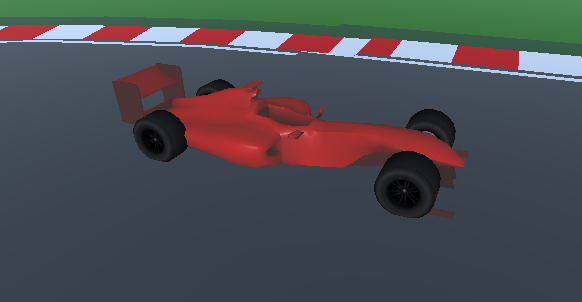
\includegraphics[height=6cm, width=10cm]{images/formula}
    \caption{Изглед модела формуле}
    \label{Image 1:}
\end{figure}

\indentМодел подлоге (терен компонента) има текстуру зелене боје и представља позадину на којој ће касније бити компоненте за стазу.\\
\indentЗа модел стазе коришћен је бесплатан Unity Asset (\href{https://assetstore.unity.com/packages/3d/environments/roadways/modular-lowpoly-track-roads-free-205188}{линк}) и представља компоненте од којих је направљен жељени изглед стазе.\\
\indentУ оквиру обог пројекта постоје три стазе које су одвојене и на којима се тренирају модели:
\begin{itemize}
  \item Стаза за кретање само на лево
  \item Стаза за кретање само на десно
  \item Стаза са комбинованим скретањима на десно или лево - најкомпликованија
\end{itemize}
\indentУ наставку ће бити илустративно приказане све врсте набројаних стаза редом како су набројане: 

\begin{center}
    \centering 
    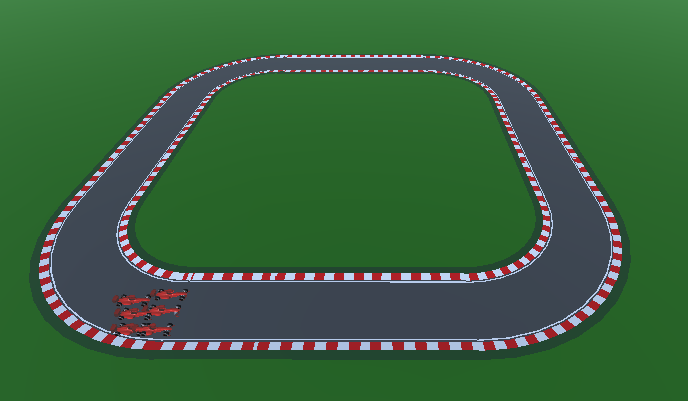
\includegraphics[height=8cm, width=12cm]{images/track1}
     \captionof{figure}{Стаза са скретањима на лево}
\end{center}
\vspace{0.5cm}
\begin{center}
    \centering 
    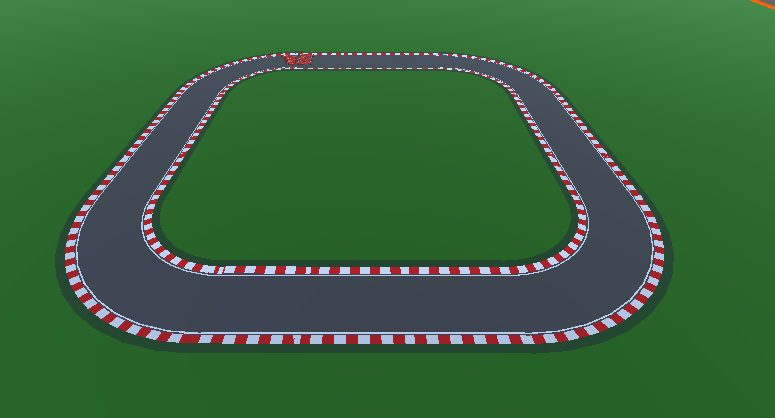
\includegraphics[height=8cm, width=12cm]{images/track2}
     \captionof{figure}{Стаза са скретањима на десно}
\end{center}

\begin{center}
    \centering 
    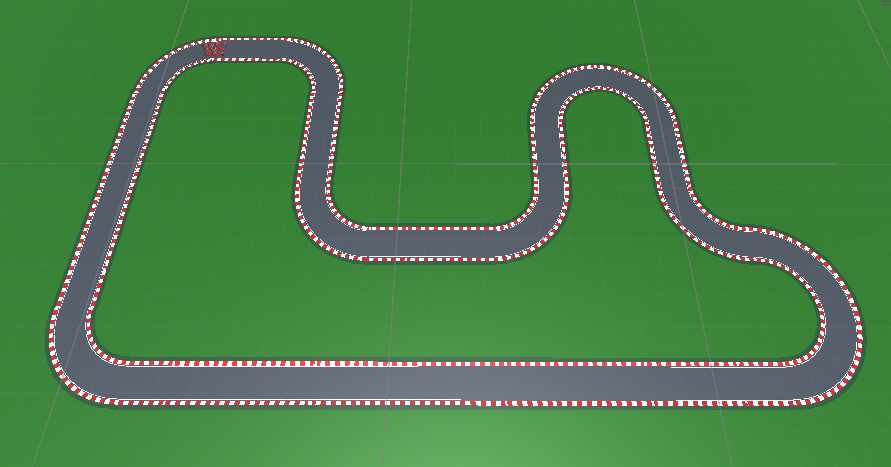
\includegraphics[height=8cm, width=12cm]{images/track3}
     \captionof{figure}{Стаза са комбинованим скретањима}
\end{center}
\vspace{0.5cm}
    \begin{center}
    \centering 
    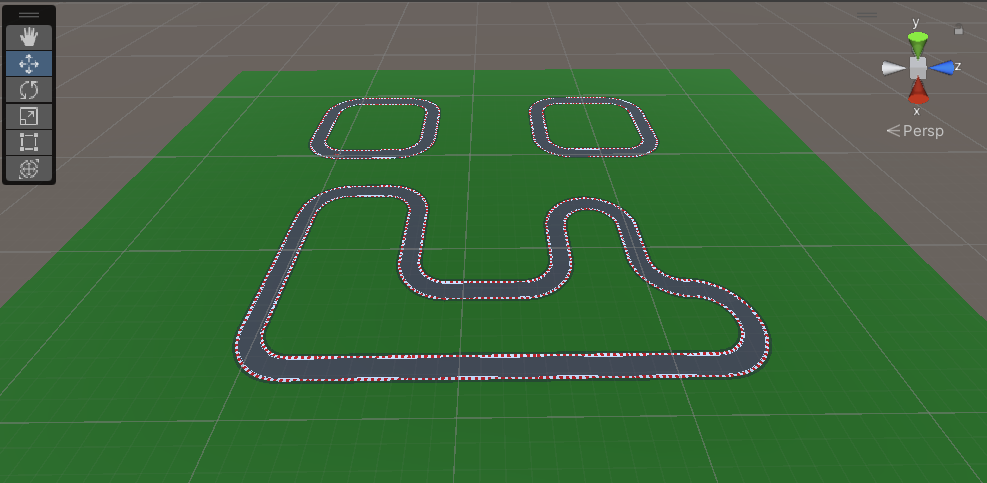
\includegraphics[height=11cm, width=15cm]{images/allTracks}
     \captionof{figure}{Све стазе у једном приказу}
\end{center}
\vspace{0.7cm}
Оно што је изостављено на претходним сликама, а што ће бити приказано у наставку јесу исте стазе али са приказаним зидовима (Walls) и контролним тачкама (Checkpoints) који су након покретања невидљиви али се виде приликом израде пројекта. Они служе за то да би се формула могла наградити уколико додирне исправан checkpoint или казнити (наградити негативно) уколико додирне зид или пограшну контролну тачку (Checkpoint). 
\begin{center}
    \centering 
    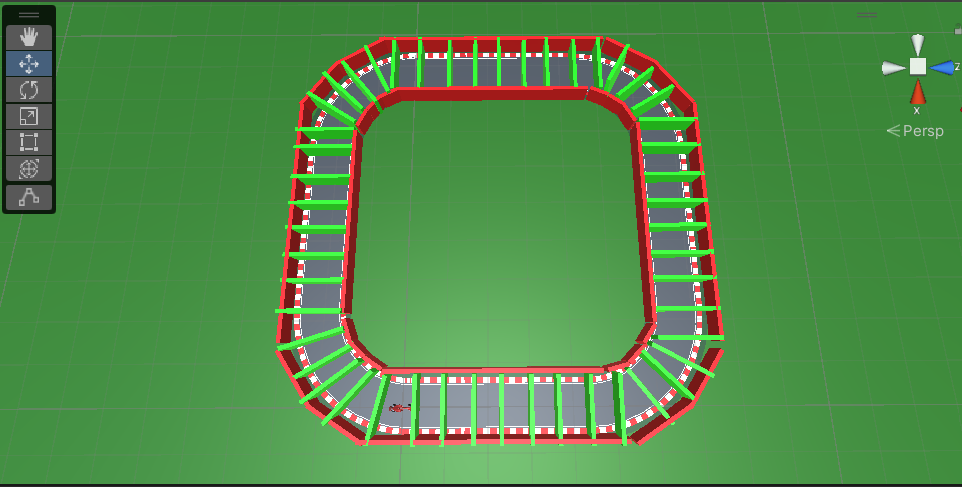
\includegraphics[height=7cm, width=12cm]{images/track1Walls}
     \captionof{figure}{Стаза лево + зидови и checkpoints}
\end{center}
\vspace{0.5cm}
\begin{center}
    \centering 
    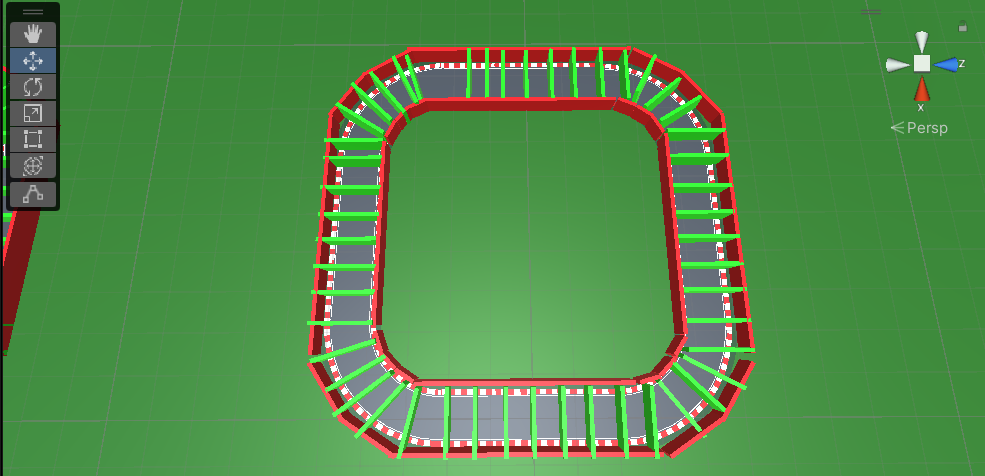
\includegraphics[height=7cm, width=12cm]{images/track2Walls}
     \captionof{figure}{Стаза десно + зидови и checkpoints}
\end{center}
\begin{center}
    \centering 
    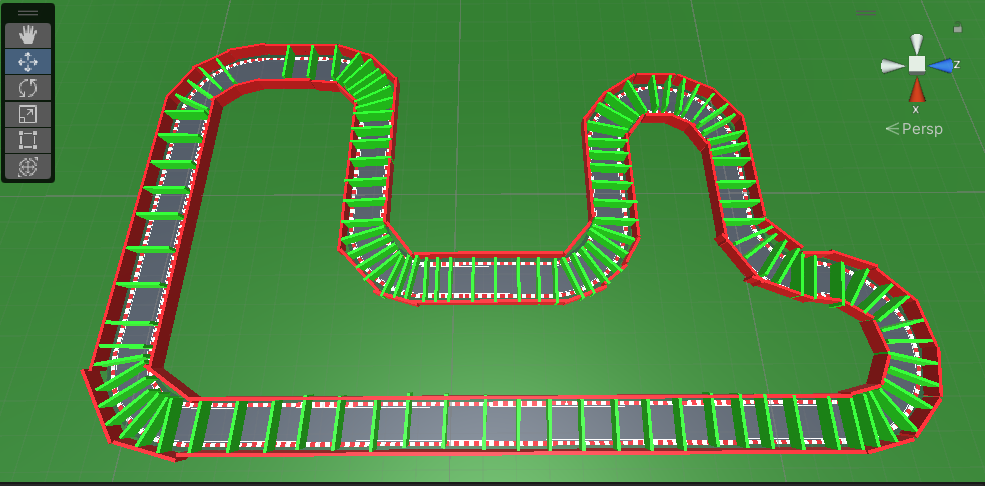
\includegraphics[height=8cm, width=12cm]{images/track3Walls}
     \captionof{figure}{Велика стаза + зидови и checkpoints}
\end{center}
\vspace{0.5cm}
\begin{center}
    \centering 
    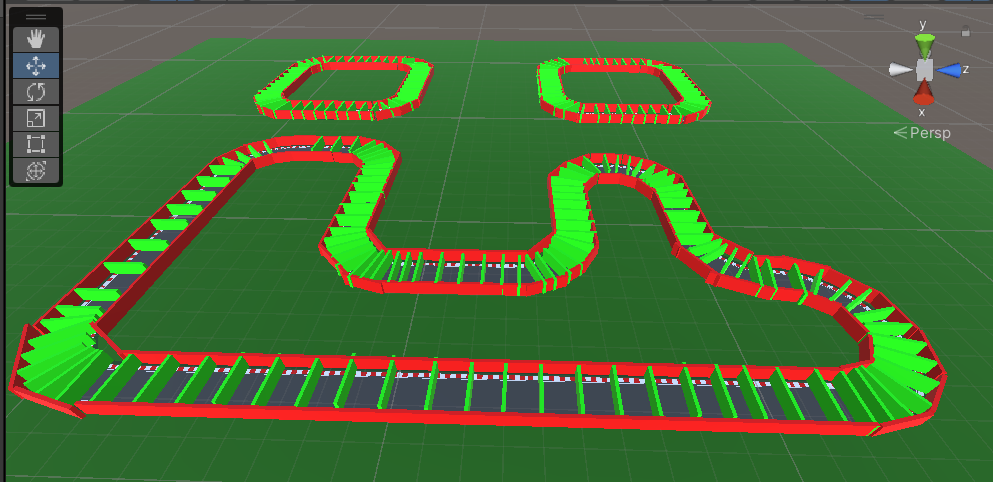
\includegraphics[height=11cm, width=15cm]{images/allTracksWalls}
     \captionof{figure}{Све стазе + зидови и checkpoints}
\end{center}


\newpage
\section{Опис функционалности модела формуле}
Функционалност модела формуле је дефинисана кроз датотеку carDriver.cs и carDriverPlayer.cs (C\# скрипте) чији ће садржај бити објашњен у наставку. Треба напоменути да се у овим датотекама не налази имплементација за учење подстицајем. Њихов садржај ће бити накнадно објашњен у секцији за опис имплементације учења подстицајем.\\\\
Опис садржаја датотеке \texttt{carDriver.cs}:\\
- садржи класу \texttt{carDriver} у којој се дефинишу следеће променљиве (за брзину, убрзање, кочење, угаону брзину, ... као и RigidBody променљива која омогућује објекту да реагује на физику у реалном времену):
\begin{center}
    \centering 
    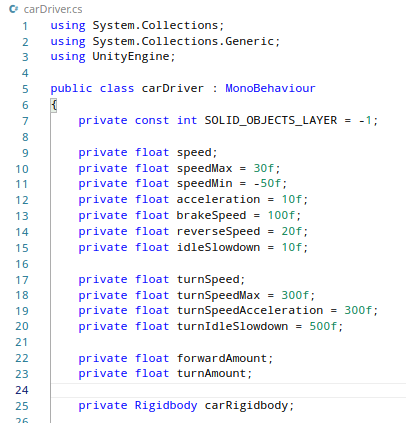
\includegraphics[height=11cm, width=10cm]{images/csDriver_fields.png}
     \captionof{figure}{Дефиниција променљивих у carDriver класи}
\end{center}
\vspace{0.5cm}
\indentКласа carDriver садржи следеће функције: 
\begin{itemize}
  \item \mycode{private void Awake()} - инстанцира се променљива \texttt{carRigidBody}
  \item \mycode{private void FixedUpdate()} - позива се при сваком фиксном фрејму и садржи највећи део понашања самог објекта формуле
  \item \mycode{private void OnCollisionEnter(Collision collision)} - региструје колизију са другим објектом
  \item \mycode{public void SetInputs(float forwardAmount, float turnAmount)} - позива се када играч управља објектом формуле
  \item \mycode{public void ClearTurnSpeed()} - подешава угаону брзину на нула
  \item \mycode{public float GetSpeed()} - враћа тренутну брзину
  \item \mycode{public void SetSpeedMax(float speedMax)} - подешава максималну брзину
  \item \mycode{public void SetTurnSpeedMax(float turnSpeedMax)} - подешава максималну угаону брзину
  \item \mycode{public void SetTurnSpeedAcceleration(float turnSpeedAcceleration)} - подешава угаоно убрзање
  \item \mycode{public void StopCompletely()} - зауставља кретање модела постављањен брзине и угаоне брзине на нула
  \item \mycode{public Vector3 GetRigidbodyVelocity()} - враћа брзину (velocity) RigidBody објекта
\end{itemize}
\vspace{0.5cm}
Опис садржаја датотеке \texttt{carDriverPlayer.cs}:\\
- садржи класу \texttt{carDriverPlayer} у којој се дефинише променљива типа carDriver. Класа \texttt{carDriverPlayer} омогућује да се од играча региструју команде и проследе објекту \texttt{carDriver} класе. Саджај ове класе ће бити приказан у потпуности на наредној слици јер је имплементација кратка:
\begin{center}
    \centering 
    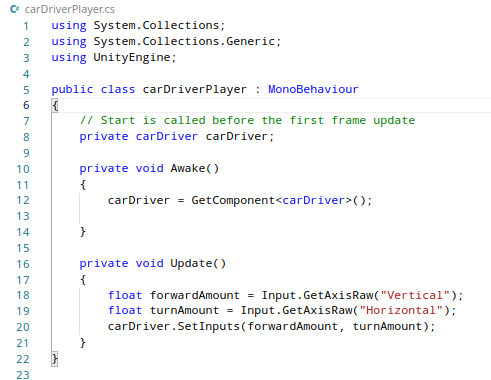
\includegraphics[height=9cm, width=10cm]{images/carDriverPlayer.png}
     \captionof{figure}{Садржај carDriverPlayer.cs датотеке}
\end{center}
\vspace{0.5cm}
\indentКласа \texttt{carDriverPlayer} садржи следеће функције: 
\begin{itemize}
  \item \mycode{private void Awake()} - инстанцира се променљива \texttt{carDriver}
  \item \mycode{private void Update()} - позива се при сваком фрејму и региструје команде (улазе) које задаје играч и прослеђује их \texttt{SetInputs} функцији \texttt{carDriver} објекта.
\end{itemize}

\newpage
\section{Опис имплементације учења подстицајем}
Учење подстицајем (Reinforcement Learning) се састоји од цикличног процеса разматрања, одлуке, акције и награде као што је то приказано на слици испод:
\begin{center}
    \centering 
    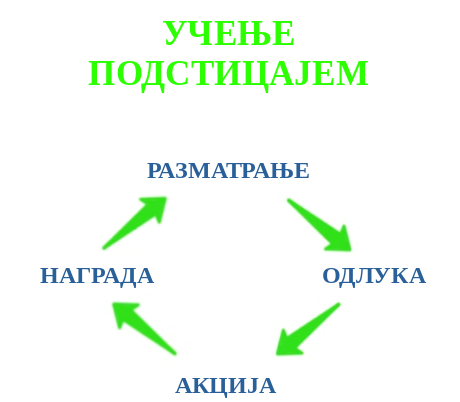
\includegraphics[height=9cm, width=10cm]{images/RL-cycle.png}
     \captionof{figure}{Процес учења подстицајем}
\end{center}
\vspace{0.5cm}
Кроз све ове процесе потребно је да прође модел који тренирамо како би исправно научио да заврши стазу.\\\\
Имплементација везана за тренирање модела садржана је у следеће три датотеке:
\begin{itemize}
  \item \texttt{CheckpointSingle.cs} - имплементација за једну контролну тачку
  \item \texttt{TrackCheckpoints.cs} - имплементација за све контролне тачке на стази
  \item \texttt{carDriverAgent.cs} - имплементација агента - формуле (модела који учи)
\end{itemize}
\vspace{0.5cm}
\indentДа бисмо наставили са објашњавањем техника коришћених при имплементацији алгоритма машинског учења, прво је потребно да размотримо принцип контролних тачака и разлог због којих оне постоје. Наиме, постојање контролних тачака на одређеном растојању по стази прикупља информације о томе где се модел који учи тренутно налази и на основу тога му даје одређену награду било позитивну било негативну. Циљ модела је да максимизира награду и на основу тога се заправо одвија његово учење. Алгоритам за сваки покренути модел води рачуна која је једина исправна контролна тачка кроз коју модел треба проћи како би добио награду и ако заиста и прође кроз њу биће награђен и то ће се сматрати као напредак. Такође, негативна награда постоји и ако модел удари у зид тј. ако скрене са стазе.\\\\
Опис садржаја датотеке \texttt{CheckpointSingle.cs}:\\
- садржи класу \texttt{CheckpointSingle} у којој се дефинише променљива типа \texttt{TrackCheckpoints}. Саджај ове класе ће бити приказан у потпуности на наредној слици јер је имплементација кратка:
\begin{center}
    \centering 
    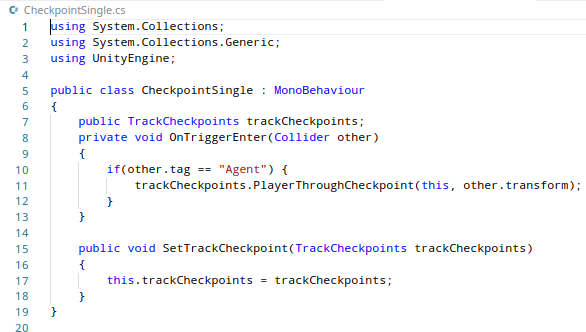
\includegraphics[height=10cm, width=15cm]{images/checkPointSingle.png}
     \captionof{figure}{Садржај CheckpointSingle.cs датотеке}
\end{center}
\vspace{0.5cm}
\indentКласа \texttt{CheckpointSingle} садржи следеће функције: 
\begin{itemize}
  \item \mycode{private void OnTriggerEnter(Collider other)} - региструје ако агент додирне контролну тачку и прослеђује ту информацију и податке о агенту објекту \texttt{TrackCheckpoints} преко његове функције \texttt{PlayerThroughCheckpoint}
  \item \mycode{public void SetTrackCheckpoint(TrackCheckpoints trackCheckpoints)} - служи за иницијализацију променљиве типа \texttt{TrackCheckpoints}
\end{itemize}
\vspace{0.5cm}
Опис садржаја датотеке \texttt{TrackCheckpoints.cs}:\\
Класа \texttt{TrackCheckpoints} садржи следећа поља: 
\begin{itemize}
  \item \mycode{public event EventHandler<CarCheckpointEventArgs> OnCarCorrectCheckpoint} - слушалац догађаја дохватања исправне контролне тачке
  \item \mycode{public event EventHandler<CarCheckpointEventArgs> OnCarWrongCheckpoint} - слушалац догађаја дохватања погрешне контролне тачке
  \item \mycode{[SerializeField] public List<Transform> carTransformList} - листа података о свим агентима који уче
  \item \mycode{private List<int> nextCheckpointSingleIndexList} - листа индекса следеће исправне контролне тачке коју треба да дохвати сваки од агената агент 
  \item \mycode{private List<CheckpointSingle> checkpointSinglesList} - листа појединачних контролних тачака на стази 
  \item класа \mycode{public class CarCheckpointEventArgs} која наслеђује \texttt{EventArgs} и садржи само једно поље које представља податке о агенту који је додирнуо контролну тачку
\end{itemize}
\vspace{0.5cm}
Класа \texttt{TrackCheckpoints} садржи следеће функције: 
\begin{itemize}
  \item \mycode{private void Awake()} - проналази све контролне тачке на стази и смешта их у низ свих појединачних контролних тачака и поставља први следећи исправни индекс сваког агента на нула. Представља почетну конфигурацију.
  \item \mycode{public void PlayerThroughCheckpoint(CheckpointSingle cps, Transform tr)} - рукује догађајем када неки од агената (формула које уче) дохвати неку од контролних тачки
  \item \mycode{public void ResetCheckpoint(Transform carTransform)} - ресетује следећу исправну контролну тачку за агента чији се подаци прослеђују као аргумент
  \item \mycode{public CheckpointSingle GetNextCheckpoint(Transform carTransform)} - дохвата следећу исправну контролну тачку за агента чији се подаци прослеђују као аргумент
\end{itemize}


Опис садржаја датотеке \texttt{carDriverAgent.cs}:\\
- садржи \texttt{carDriverAgent} класу која наслеђује класу \texttt{Agent} из ML-Agents пакета
Класа \texttt{carDriverAgent} садржи следећа поља: 
\begin{itemize}
  \item \mycode{[SerializeField] public TrackCheckpoints trackCheckpoints} - податак о свим контролним тачкама на стази
  \item \mycode{[SerializeField] public Transform spawnPosition} - садржи податке о положају агента приликом рестартовања
  \item \mycode{public event EventHandler OnCarCorrectCheckpoint} - слушалац догађаја за пролазак кроз исправну контролну тачку
  \item \mycode{public event EventHandler OnCarWrongCheckpoint} - слушалац догађаја за пролазак кроз погрешну контролну тачку 
  \item \mycode{private carDriver carDriver} - садржи све податке и функционалности обичног агента 
\end{itemize}
\vspace{0.5cm}
Класа \texttt{TrackCheckpoints} садржи следеће функције: 
\begin{itemize}
  \item \mycode{private void Awake()} - инстанцира се објекат типа \texttt{carDriver}
  \item \mycode{private void Start()} - подешавање почетне конфигурације за контролне тачке
  \item private void TrackCheckpoints\_OnCarWrongCheckpoint(object sender, TrackCheckpoints.CarCheckpointEventArgs e) - давање негативне награде ако је агент дохватио погрешну контролну тачку
  \item private void TrackCheckpoints\_OnCarCorrectCheckpoint(object sender, TrackCheckpoints.CarCheckpointEventArgs e) - давање позитивне награде ако је агент дохватио погрешну контролну тачку
  \item \mycode{public override void OnEpisodeBegin()} - дешавање на почетку новог круга учења - ресет на почетну конфигурацију
  \item \mycode{public override void CollectObservations(VectorSensor sensor)} - функција за разматрање у оквиру ML-Agents пакета 
  \item \mycode{public override void OnActionReceived(ActionBuffers actions)} - подешавање исхода акције предузетих као резултат донесене одлуке
  \item \mycode{public override void Heuristic(in ActionBuffers actionsOut)} - функција за мануелно управљање од стране играча
  \item \mycode{public void OnTriggerEnter(Collider other)} - детектује додир са зидом и даје негативну награду и завршава круг
  \item \mycode{public void OnTriggerStay(Collider other)} - слично као претходна функција само што не завршава круг
\end{itemize}
\vspace{0.5cm}
Сам процес учења може се пратити у конзоли тако што се исписује награда коју агенти добијају у сваком кругу тренирајући заједно. Један такав испис приказан је на следећој слици:
\begin{center}
    \centering 
    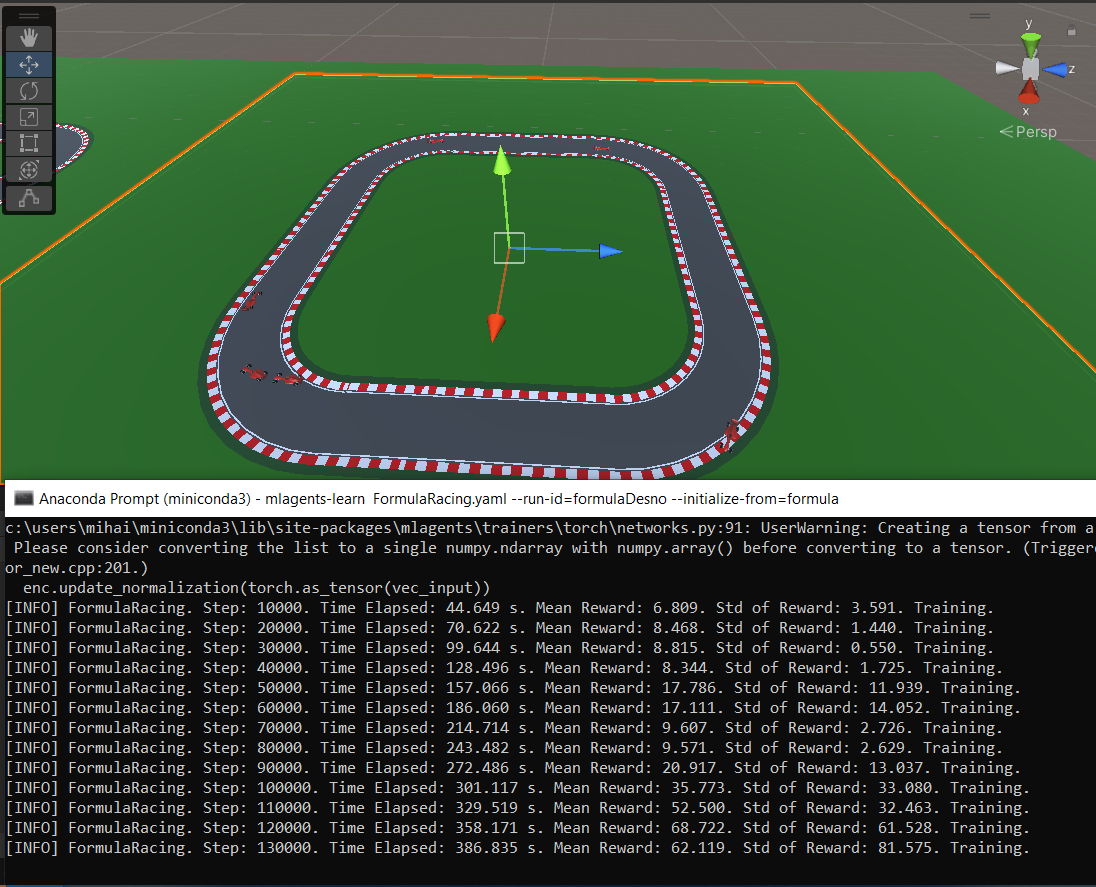
\includegraphics[height=13cm, width=16cm]{images/rewardOutput.png}
     \captionof{figure}{Испис у току тренирања модела}
\end{center}
\vspace{0.5cm}
Такође, битна компонента самог пројетка јесте .yaml датотека која се у нашем случају назива FormulaRacing.yaml и у њој се налази конфигурација коју у позадини користи алгоритам учења подстицајем. Ту нпр. можемо подесити максимаан број итерација кроз које модел пролази приликом једног учења кретања. Садржај датотеке је приказан на следећој слици:
\begin{center}
    \centering 
    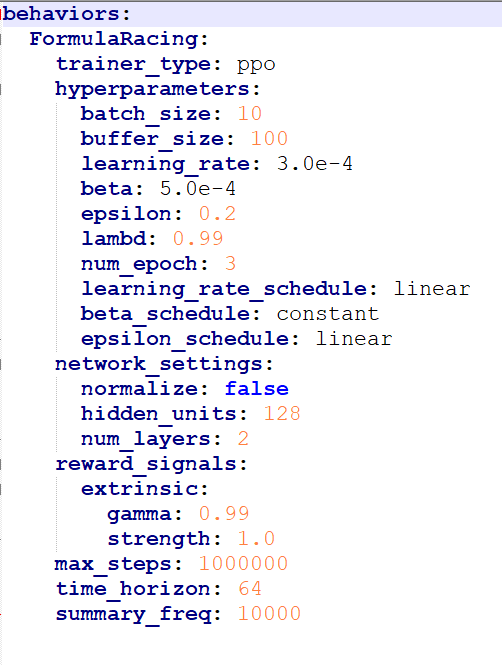
\includegraphics[height=10cm, width=10cm]{images/yamlFile.png}
     \captionof{figure}{Приказ конфигурационог .yaml фајла}
\end{center}
\vspace{0.5cm}
Након што модел заврши процес учења генерише се .onnx фајл у коме је садршан "мозак" нашег модела тј. оно што је он у току тренирања научио. Тај "мозак" остаје сачуван и после се може учитати како би се демонстрирало то што је модел научио. Такоће се може научени алгоритам на једној стази покренути на сасвим другој како би се провјериле способности тренираног агента на тзв. "непознатом терену". 




\newpage
\section{Литература}
\begin{itemize}
  \item \url{https://elektrotehnika.github.io/ml/}
  \item YouTube туторијали за коришћење ML-Agents пакета у оквиру Unity окружења - \href{https://www.youtube.com/watch?v=zPFU30tbyKs&list=PLzDRvYVwl53vehwiN_odYJkPBzcqFw110&index=1}{линк1}, \href{https://www.youtube.com/watch?v=2X5m_nDBvS4&list=PLzDRvYVwl53vehwiN_odYJkPBzcqFw110&index=4}{линк2}
  \item \url{https://assetstore.unity.com/}
  \item \url{https://stackoverflow.com/}
  \item Интернет
\end{itemize}


\end{document}
